\documentclass[a4paper, 10pt]{article}
\usepackage[utf8]{inputenc}
\usepackage[spanish]{babel}
\usepackage{hyperref}
\usepackage{tabularx}
\usepackage{inconsolata}
\usepackage{enumitem}
\usepackage{graphicx}
\usepackage{subfigure}
\usepackage{listings}
\usepackage{color}
\usepackage{appendix}

\usepackage{multirow}

\newcommand{\cabeceraSI}[2]{
	\begin{center}
	\begin{tabularx}{\textwidth}{|c c|X|X|X|X}
	\hline
	  \multicolumn{2}{|c|}{\multirow{3}{*}{
\includegraphics[scale=0.10]{../uam.png}}} & \multicolumn{4}{c|}{\bfseries Escuela Politécnica Superior}\\
	  & & \multicolumn{4}{c|}{\bfseries Ingeniería Informática}\\
	  & & \multicolumn{4}{c|}{\bfseries Prácticas de Sistemas Informáticos 2}\\
	\hline
	  \multicolumn{1}{|c|}{\textbf{Grupo}} & 2401 & \multicolumn{1}{|c|}{\textbf{Práctica}} & \multicolumn{1}{>{\centering\arraybackslash}X|}{#1} & \multicolumn{1}{>{\bfseries\centering\arraybackslash}X|}{Fecha} & \multicolumn{1}{c|}{#2}\\
	\hline
	  \multicolumn{2}{|c|}{\textbf{Alumno}} & \multicolumn{4}{l|}{Kasner Tourné, Cristina}\\
	\hline
	  \multicolumn{2}{|c|}{\textbf{Alumno}} & \multicolumn{4}{l|}{Guridi Mateos, Guillermo}\\
	\hline
	\end{tabularx}
	\end{center}
}

\definecolor{mygreen}{rgb}{0,0.6,0}
\definecolor{mygray}{rgb}{0.5,0.5,0.5}
\definecolor{mymauve}{rgb}{0.58,0,0.82}

\lstset{ %
	backgroundcolor=\color{white},   % choose the background color; you must add \usepackage{color} or \usepackage{xcolor}
	basicstyle=\footnotesize,        % the size of the fonts that are used for the code
	breakatwhitespace=false,         % sets if automatic breaks should only happen at whitespace
	breaklines=true,                 % sets automatic line breaking
	captionpos=b,                    % sets the caption-position to bottom
	commentstyle=\color{mygreen},    % comment style
	deletekeywords={...},            % if you want to delete keywords from the given language
	escapeinside={\%*}{*)},          % if you want to add LaTeX within your code
	extendedchars=true,              % lets you use non-ASCII characters; for 8-bits encodings only, does not work with UTF-8
	frame=single,                    % adds a frame around the code
	keepspaces=true,                 % keeps spaces in text, useful for keeping indentation of code (possibly needs columns=flexible)
	keywordstyle=\color{blue},       % keyword style
	language=Octave,                 % the language of the code
	morekeywords={*,...},            % if you want to add more keywords to the set
	numbers=left,                    % where to put the line-numbers; possible values are (none, left, right)
	numbersep=5pt,                   % how far the line-numbers are from the code
	numberstyle=\tiny\color{mygray}, % the style that is used for the line-numbers
	rulecolor=\color{black},         % if not set, the frame-color may be changed on line-breaks within not-black text (e.g. comments (green here))
	showspaces=false,                % show spaces everywhere adding particular underscores; it overrides 'showstringspaces'
	showstringspaces=false,          % underline spaces within strings only
	showtabs=false,                  % show tabs within strings adding particular underscores
	stepnumber=2,                    % the step between two line-numbers. If it's 1, each line will be numbered
	stringstyle=\color{mymauve},     % string literal style
	tabsize=2,                       % sets default tabsize to 2 spaces
	title=\lstname                   % show the filename of files included with \lstinputlisting; also try caption instead of title
}

\makeatletter
\def\@seccntformat#1{%
  \expandafter\ifx\csname c@#1\endcsname\c@section\else
  \csname the#1\endcsname\quad
  \fi}
\makeatother

\newcommand{\tabitem}{\vspace{1mm}~~\llap{\textbullet}~~}

\hypersetup{
    colorlinks=true,
    citecolor=black,
    linkcolor=black,
    urlcolor=blue
}

%% Titulo y autores
\title{Sistemas Informáticos 2\\Práctica 1b}
\author{Cristina Kasner Tourné\and Guillermo Guridi Mateos}
\date{\today}

%% Documento
\begin{document}

\cabeceraSI{1b}{4/03/2015}

\section{Cuestión 1}\texttt{\textbf{VisaDAOLocal.java}}

	En este archivo se especifican los métodos que van a poder ser llamados sobre el EJB que implemente la interfaz \texttt{VisaDAOLocal}.

	Vemos que tiene la etiqueta \texttt{@Local} , que significa:
	\begin{itemize}
		\item Debe ejecutarse en la misma Maquina Virtual Java del EJB al que accede
		\item Puede ser un componente web u otro EJB
		\item Para el cliente local, la localización del EJB al que accede no es transparente
	\end{itemize}


\section{Ejercicio 1}

	Para ajustar los métodos a la interfaz hemos quitado la etiqueta de \texttt{synchronize} ya que no se utilizan en los métodos especificados en \texttt{VisaDAOLocal}.

	También hemos cambiado el retorno del método \texttt{getPagos}, antes devolvía \texttt{ArrayList} y ahora devuelve \texttt{PagoBean []} para respetar las declaraciones de \texttt{VisaDAOLocal}.

	\section{Ejercicio 2}
	Hemos eliminado de los \texttt{servlets} todo lo referente a los \textit{Web Services} (que estaban en los respectivos métodos \texttt{ProcessRequest} del cliente) ya que ahora hacemos uso del EJB que hace uso de la interfaz \texttt{VisaDAOLocal}.

	Entre las cosas que hemos tenido que quitar están los imports del paquete \texttt{javax.xml.ws} y todo el código que obtenía \texttt{VisaDAO} a través de un servicio y le asignaba una dirección de recurso dinámicamente. Por supuesto, tan bien borramos el ya no necesario parámetro de \texttt{web.xml} que especificaba las rutas al servidor.

	En \texttt{getPagos} hemos vuelto a cambiar el tipo de retorno para que coincida con la declaración que hay en \texttt{VisaDAOLocal}.


\pagebreak

\section{Cuestión 2}
	Vemos que en el archivo \texttt{application.xml} hay dos módulos:
	\begin{itemize}
		\item Uno que contiene los EJBs (parte `servidor').
		\item En el otro se declara la parte web de la aplicación indicando el \texttt{.war} del cliente , y la dirección en la que será desplegada (\texttt{/P1-ejb-cliente})
	 \end{itemize}
	 
	 Cuando ejecutamos el comando \texttt{jar -tvf} vemos que nos muestra la tabla de contenidos del archivo al que se lo hemos aplicado. Vamos a explicar el caso del \texttt{.ear}. Contiene 4 archivos:

	 \begin{itemize}
	 	\item \texttt{application.xml}, del que ya hemos hablado
	 	\item \texttt{MANIFEST.MF} , que contiene información sobre la versión de \texttt{ant} usada para la empaquetación.
	 	\item \texttt{P1-ejb-cliente.war}, que es el cliente empaquetado.
	 	\item \texttt{P1-ejb.jar} , que es el servidor empaquetado.
	 \end{itemize} 

	 Al comprobar los contenidos de \texttt{P1-ejb.jar} encontramos los \texttt{.class} correspondientes a los EJBs, listos para ser utilizados por el cliente.

	 En cambio, al examinar los contenidos de \texttt{P1-ejb-cliente.war}, vimos que a parte de los \texttt{.class} encontrados también existían ficheros de configuración del servicio web, dentro de \texttt{WEB-INF}.
	

 \section{Ejercicio 3}
 
	 \begin{figure}[hbtp]
	 	\centering
	 	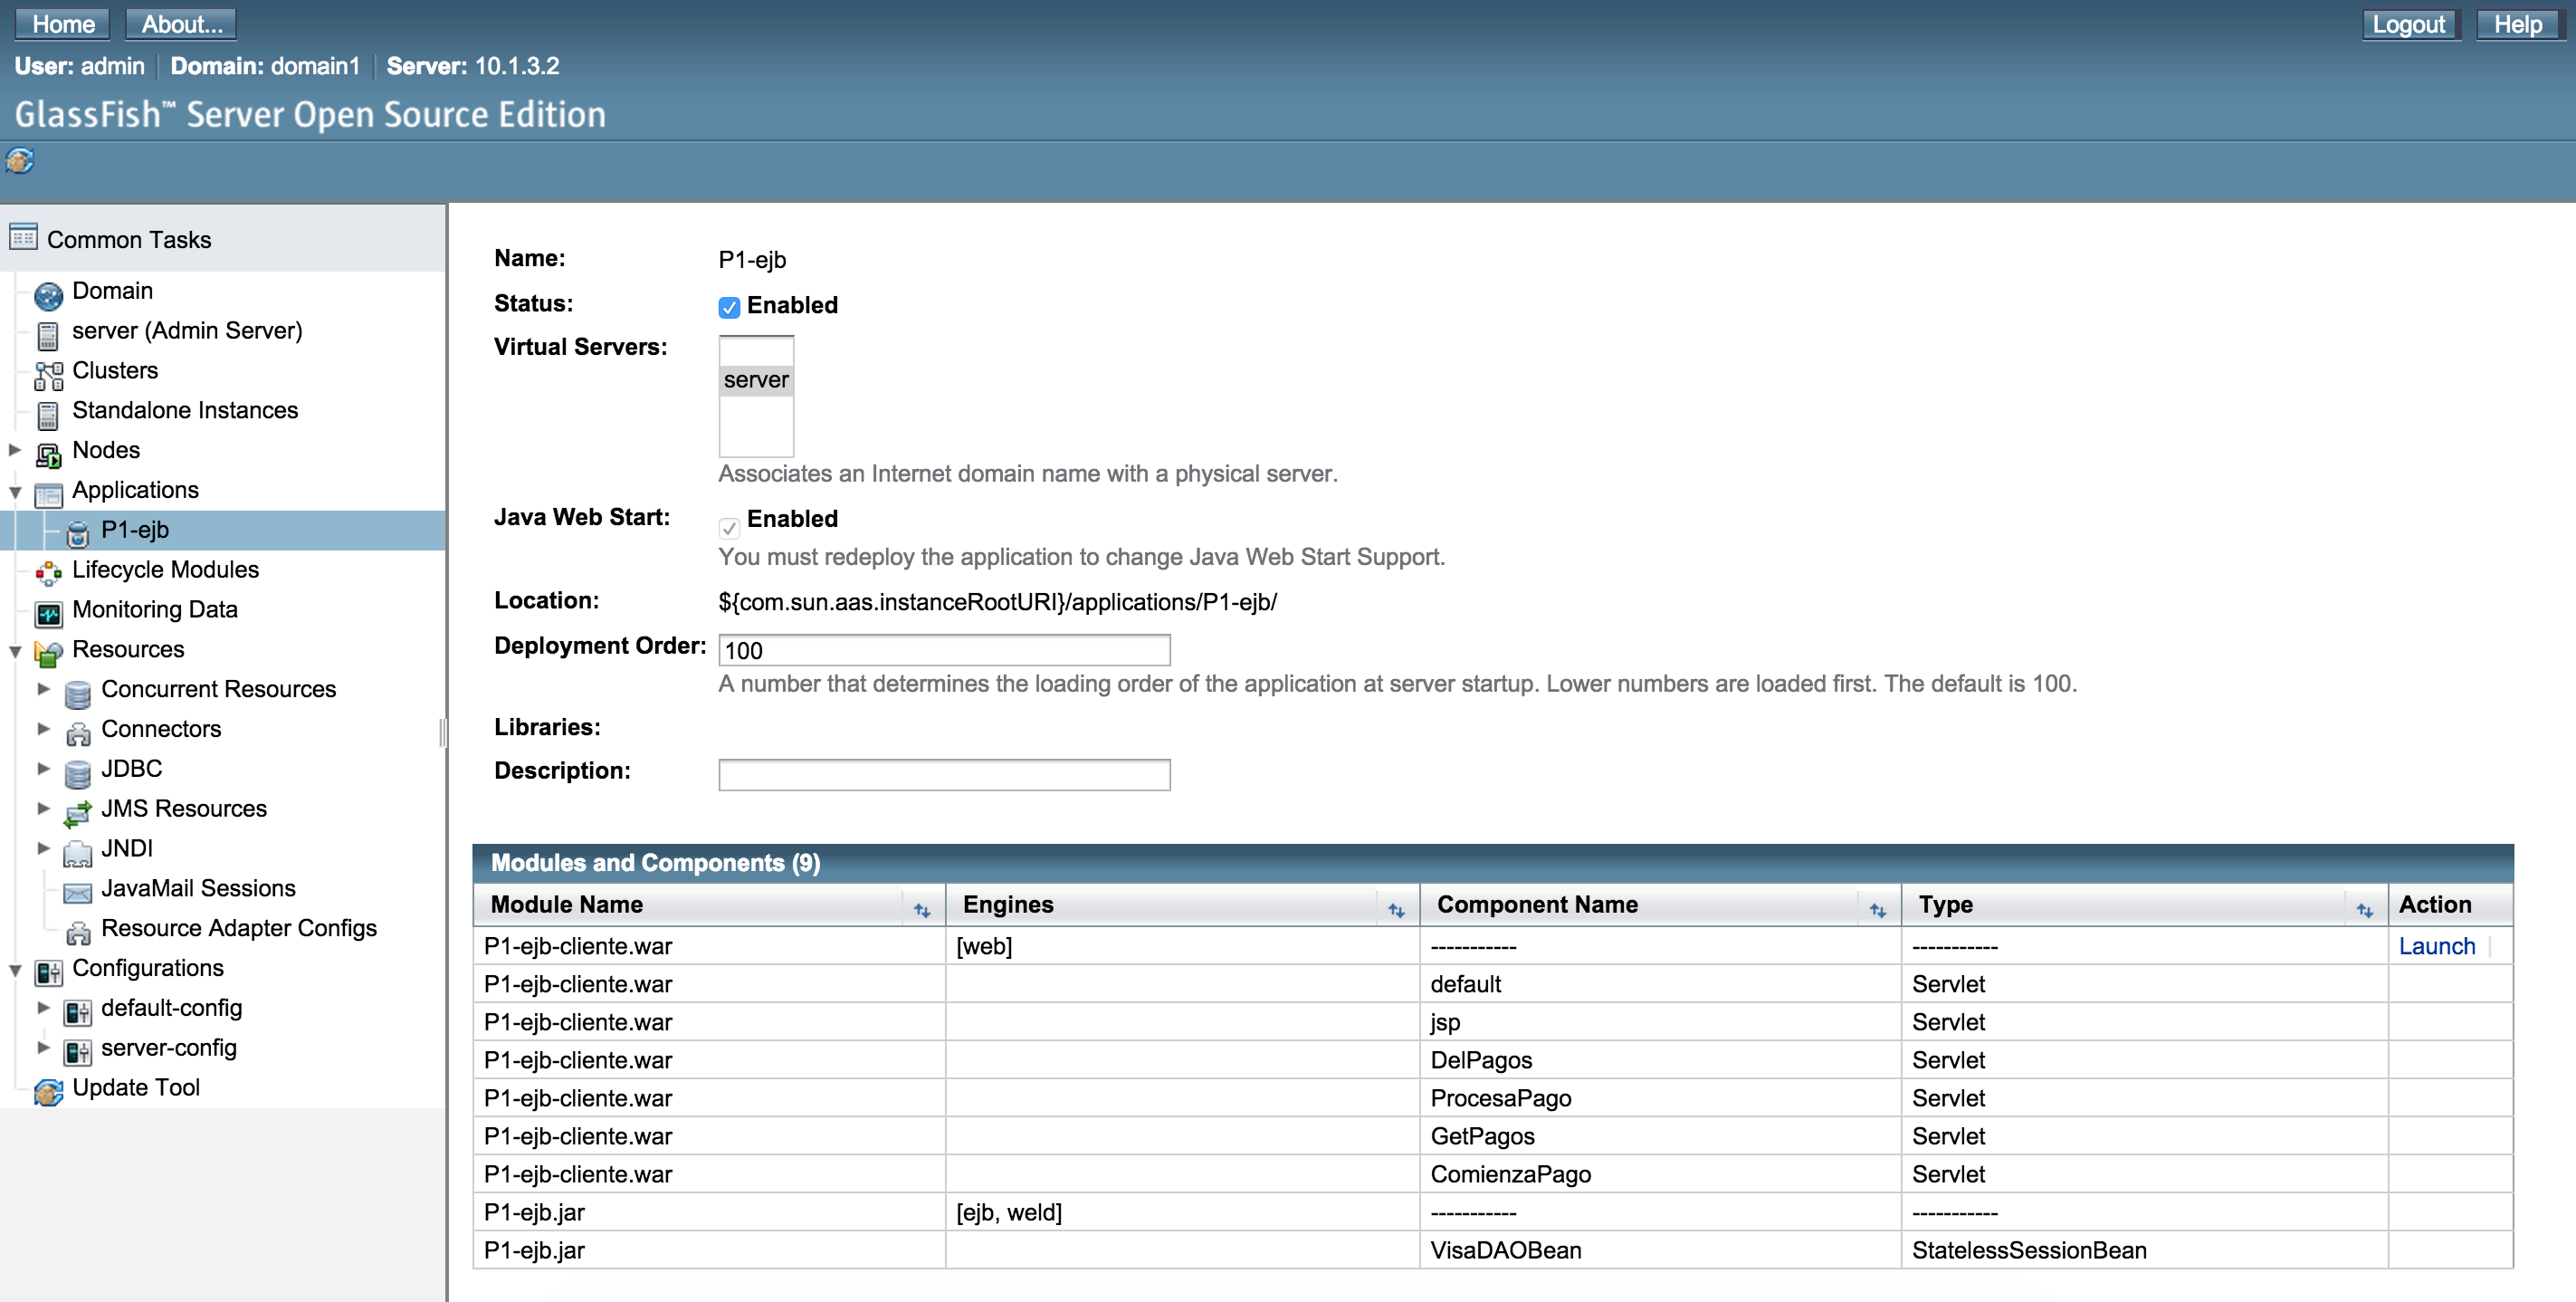
\includegraphics[width=1.1\textwidth]{pantallazos/ejercicio3.png}
	 	\caption{Comprobar en la administración de Glassfish el despliegue de la aplicación}
	 \end{figure}
 


 \section{Ejercicio 4}

	 No hubo ningún problema en las pruebas y comprobamos el estado de la base de datos a cada paso para asegurarnos de que funcionaba correctamente.

	 \begin{figure}[hbtp]
	 	\centering
	 	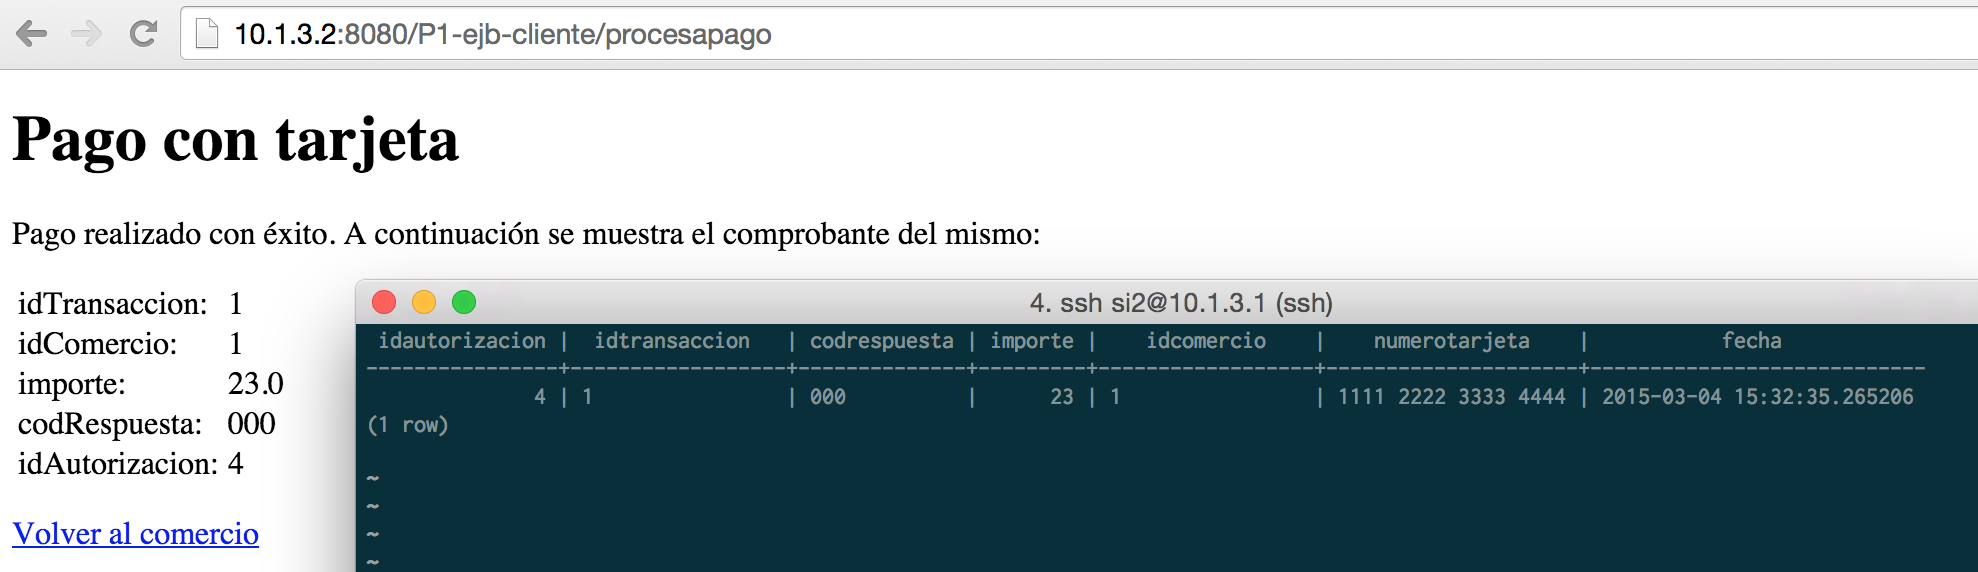
\includegraphics[width=1.1\textwidth]{pantallazos/ejercicio4.png}
	 	\caption{Muestra de un pago realizado a través de EJBs}
	 \end{figure}



 \section{Ejercicio 5}
	 \begin{itemize}
	 	\item Archivo \texttt{ TarjetaBean.java}
	 	
	 	
	 	 Además de añadir saldo como atributo hemos añadido los métodos \texttt{getSaldo} y \texttt{setSaldo}.
	 	 
	 	 
	 	 \item Archivo \texttt{ VisaDAOBean.java}
	 	 
	 	 
	 	 Hemos creado las dos consultas y hemos modificado el método \texttt{realizaPago} para que ejecute las dos consultas anteriores usando los \textit{prepared statements}.
	 	 
	 	 Al contrario que las otras consultas que se ejecutan en \texttt{realizaPago}, estas no dan la opción de no usar el \textit{prepared}, ya que solo hemos construido ese tipo de query. El resto de querys siguen utilizando ambos métodos.
	 	  	 
	 	 Para lanzar la excepción en caso de que algo falle hemos añadido un \texttt{String} que explica la razón por la que ha fallado y se los mandamos al cliente junto con la \texttt{EJBException}.
	 	 
	 	 \item Archivo \texttt{ProcesaPago}
	 	 
	 	 Hemos capturado la excepción con un bloque \texttt{try / catch} que llama a \texttt{enviaError}.
	 \end{itemize}
 
\pagebreak
 


\section{Ejercicio 6}
	\begin{figure}[htbp]
		\centering	
		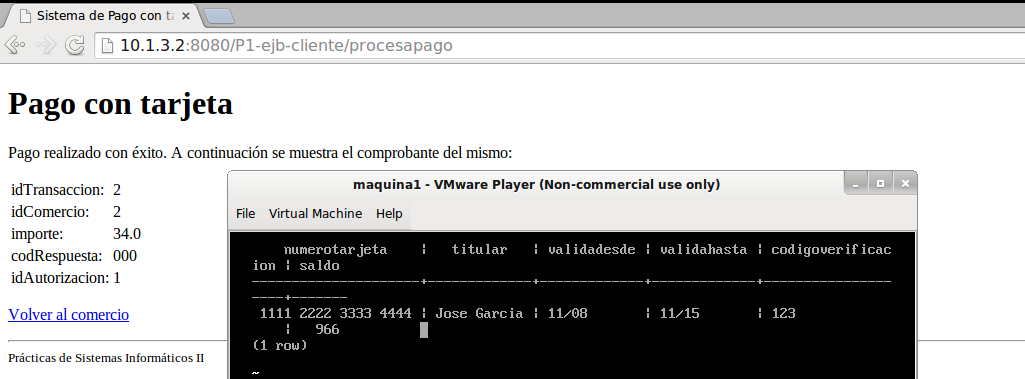
\includegraphics[width=1\textwidth]{pantallazos/ejercicio6a.png}
		\caption{Pago realizado sobre la base de datos recien inicializada (Todas las tarjetas tenían saldo 1000)}
	\end{figure}
 	
 	\begin{figure}[htbp]
		\centering	
		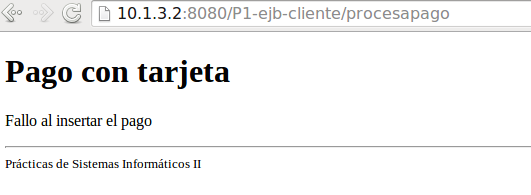
\includegraphics[width=1\textwidth]{pantallazos/ejercicio6b.png}
		\caption{Resultado de un intento de pago con la misma id de transacción y de comercio}
	\end{figure}



\section{Ejercicio7}
	Creamos manualmente a través de la interfaz de administración de Glassfish la factoría de mensajes aunque dudamos un poco al no coincidir completamente los nombres de los campos que hay en la captura de pantalla del enunciado con lo que veíamos nosotros. En concreto cambiaba la etiqueta del campo \textit{Pool Name} por \textit{JNDI Name}. Pudimos comprobar en ejercicios posteriores que era lo mismo ya que las referencias funcionaban.

	\begin{figure}[htbp]
		\centering
		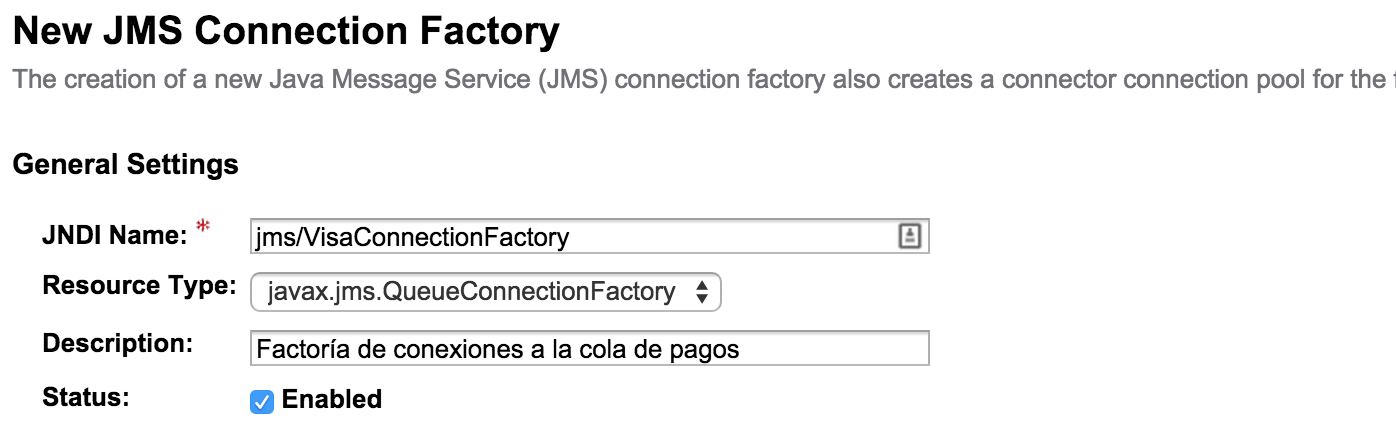
\includegraphics[width=0.7\textwidth]{pantallazos/ejercicio7.png}
	\end{figure}


\pagebreak

\section{Ejercicio8}
	Realizando tareas similares a las del ejercicio 7 no tuvimos ningún porblema creando la cola de mensajes.




\section{Ejercicio9}
 	\begin{itemize}

 		\item Archivo \texttt{sun-ejb-jar.xml}

 		Bastó añadir el siguiente fragmento dentro del ejb declarado con los datos especificados en el ejercicio 7.

 		\texttt{<mdb-connection-factory>}

      	\hspace{3em}\texttt{<jndi-name>jms/VisaConnectionFactory</jndi-name>}

      	\texttt{</mdb-connection-factory>}
 		

 		\item Archivo \texttt{VisaCancelacionJMSBean}

 		Construimos las querys de manera que solo hiciera falta la id de autorización para realizar ambas (pese a ser una sobre la tabla de pagos y la otra sobre la de tarjetas). Además, tuvimos en cuenta que se podría dar el caso de intentar cancelar un pago ya cancelado, así que la query de actualizar el código de respuesta no realiza ninguna actualizacion en caso de que el código ya haya sido actualizado.

 		Esto concuerda con la comprobación de errores que realizamos dentro del método. Despues de recibir \texttt{idAutorizacion} y colocar su valor en la query mediante un \textit{prepared statement}, ejecutamos la query y comprobamos cuantas filas a actualizado. En ningún caso será mayor que uno el número ya que una de las condiciones es de igualdad en la clave primaria. Así que puede ser 1, en cuyo caso ha actualizado un pago correctamente, o 0 en cuyo caso no ha actualizado ningún pago por no existir o por que ha sido cancelado previamente.

 		En caso de que se haya cancelado con este mensaje un pago, se procede al reembolso. El cual se efectua con una query que añade el coste del pago al saldo de la tarjeta que lo ha realizado mediante dos \textit{subquerys}.

 	\end{itemize}


\section{Ejercicio10}
 	El método que hemos usado al final, obtención de recursos JMS estáticos, tiene la ventaja de, en algunos casos, ser más eficiente que el método dinámico ya que las anotaciones que declaran que va a tener esa variable en tiempo de ejecución pueden prepararse una vez, cuando se instancie la clase en el sistema al arrancar la aplicación, mientra que la búsqueda dinámica tiene que ser llamada explicitamente, lo cual es su desventaja. En cambio el método dinámico proporciona más flexibilidad al sistema permitiendo que el nombre de la factoría de conexiones o de la cola pueda ser obtenida dinámicamente (de un archivo de configuración, de variables de entorno, de la entrada del usuario, etc...) o incluso cambiada en algún momento, al contrario que el método estático, en el que los nombres de los recursos deben saberse en tiempo de compilación al estar incluidos dentro de una anotación \texttt{@Resource}.


\section{Ejercicio11}

	No hubo que realizar cambios en ninguno de los archivos \texttt{xml} mencionados ya que ambos importan los archivos de propiedades.

	Todas las direcciones ip que tuvimos que asignar fueron las de la máquina 2 ya que la base de datos permanece intacta y aislada en la 1. Así que cambiamos las variables \texttt{as.host.mdb}, \texttt{as.host.server} y \texttt{as.host.client} a \texttt{10.1.3.2}. 

	Además, en el archivo \texttt{jms.properties} asignamos las variables \texttt{jms.factoryname}, \texttt{jms.name} y \texttt{jms.physname} a los valores \texttt{jms/VisaConnectionFactory}, \texttt{jms/VisaPagosQueue} y \texttt{VisaPagosQueue} respectivamente. (EXPLICAR PHYSNAME).



\section{Ejercicio12}
	
	Como se indicó en el mensaje posterior a la publicación de la práctica, ejecutamos el cliente jms en una de las máquinas virtuales. En nuestro caso elegimos la 10.1.3.1, ya que de esta manera la cola no estaría en la misma máquina que en la que se ejecutaba el comando.

	Por supuesto, también configuramos la variable \texttt{default\_JMS\_host} (poniendo \texttt{10.1.3.2}) en glassfish para permitir la conexión desde el exterior (ya que previamente estaba definida como \texttt{localhost}).


	Al haber desactivado el \texttt{jms-mdb}, al ejecutar el primer comando, colocamos un mensaje en una cola de la que no hay nadie sacando mensajes. Esto nos permite, momentos después ejecutar el cliente jms otra vez, esta vez pidiendo que nos liste los mensajes en la cola. Con lo que pudimos comprobar que nestro código para enviar mensajes funcionaba correctamente.

	Como habíamos enviado el número 1 como mensaje, aprovechamos que en cuanto arrancáramos \texttt{jms-mdb} lo íba a procesar, y efectuamos un pago, que al ser el primero, tomaría la id de autorización 1. Efectivamente, cuando arrancamos el procesador de mensajes, se puso manos a la obra e invalidó el pago que habíamos realizado, devolviendo el dinero a la cuenta.

	\pagebreak

	\begin{figure}[H]
		\centering
		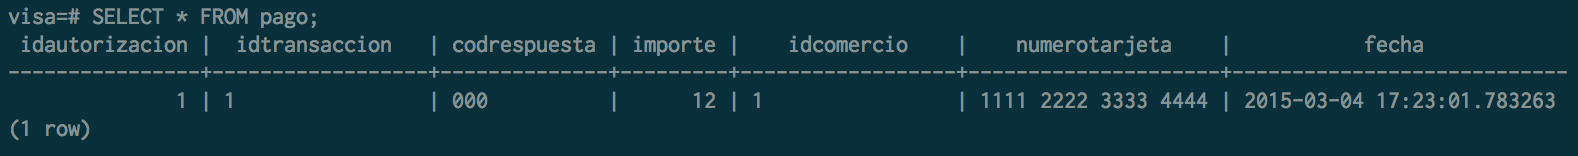
\includegraphics[width=0.9\textwidth]{pantallazos/ejercicio12a.png}
		\caption{Query para comprobar que el pago se había realizado correctamente y ver que su identificador de autorización es, como esperábamos, 1}
	\end{figure}

	\begin{figure}[htbp]
		\centering
		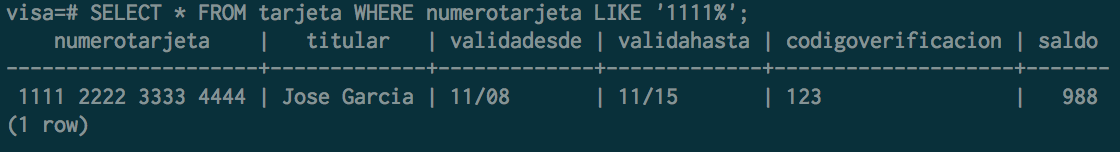
\includegraphics[width=0.9\textwidth]{pantallazos/ejercicio12b.png}
		\caption{Query para comprobar que el saldo de la tarjeta ha bajado como era esperado.}
	\end{figure}

	\begin{figure}[htbp]
		\centering
		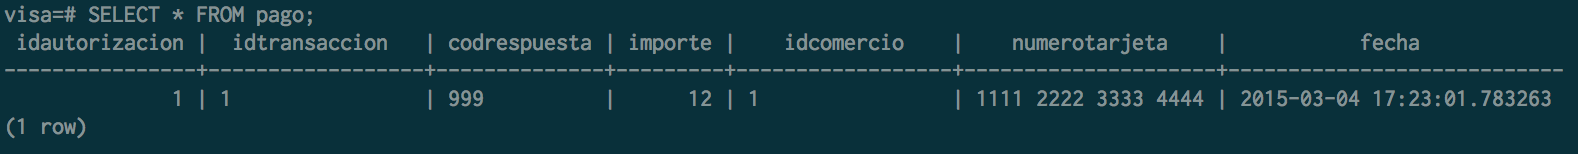
\includegraphics[width=0.9\textwidth]{pantallazos/ejercicio12c.png}
		\caption{Una vez realizada la cancelación vemos como el resultado del pago ha cambiado a 999}
	\end{figure}

	\begin{figure}[htbp]
		\centering
		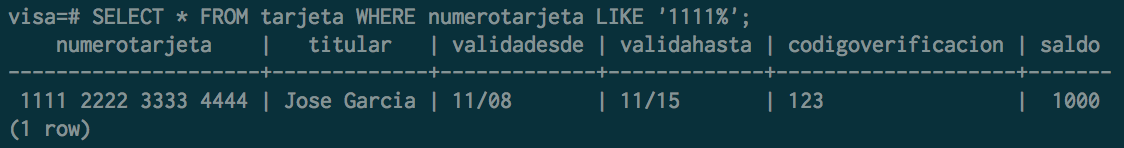
\includegraphics[width=0.9\textwidth]{pantallazos/ejercicio12d.png}
		\caption{Y también el saldo del cliente vuelve a la cantidad inicial: 1000}
	\end{figure}




%\newpage
%\appendix
%\section{Apéncices}

\end{document}